\section{Motivation and the solved problem}
\subsection{Dictionaries and hashing}
\begin{frame}
	\frametitle{The solved problem}

	\begin{block}{Dictionary}
		For arbitrary set $S$ create a representation which
		\begin{itemize}
			\item has Find running in expected constant time,
			\item has a non-trivial (sublinear) worst case guarantee for Find,
			\item consumes $O(|S|)$ memory,
			\item expected amortized running time of each operation is $\bigo(1)$.
		\end{itemize}
	\end{block}

	\begin{block}{Our approach}
		\begin{itemize}
			\item Lengths of chains are limited by a so called \emph{limit function}.			
			\item When there is a chain exceeding the value of the limit function, the hash table is rehashed using a new function.
			\item Limit functions are extracted from various universal systems.
		\end{itemize}
	\end{block}
\end{frame}

\begin{frame}
	\frametitle{Hashing -- separate chaining}
	
	\begin{block}{A simple example}
		\begin{figure}
			\begin{minipage}[t]{.45\linewidth}
				\centering
				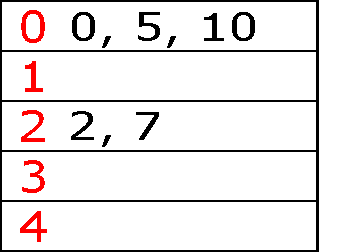
\includegraphics[width=0.55\textwidth]{sep_chain_fail.pdf}
				\caption{Hashing using function $f(x) = x \bmod 13 \bmod 5$.}
			\end{minipage}\hfill
			\begin{minipage}[t]{.45\linewidth}
				\centering
				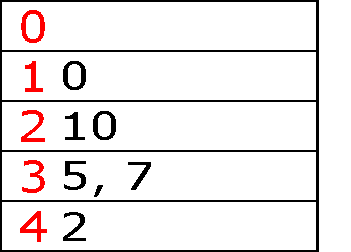
\includegraphics[width=0.55\textwidth]{sep_chain_ok.pdf}
				\caption{New hash function $f(x) = (4x + 1) \bmod 13 \bmod 5$.}
			\end{minipage}
		\end{figure}

		\begin{itemize}
			\item If there is a long chain ($0, 5, 10$), then Find is slow.
			\item Idea -- rehash using a new function. 
			\item Universal hashing is thus a must.
		\end{itemize}
	\end{block}
\end{frame}

\begin{frame}
	\frametitle{Hashing with a Worst Case Lookup}
	
	\begin{block}{Perfect hashing}
		\begin{itemize}
			\item Algorithm finds a perfect hash function for a given static set.
			\item Dynamizations of FKS scheme are known.
		\end{itemize}
	\end{block}
	
	\begin{block}{Cuckoo hashing}
		\begin{itemize}
			\item State of the art method with $\bigo(1)$ lookup.
			\item Problems with space consumption and universal systems.
		\end{itemize}
	\end{block}
	
	\begin{block}{Two-way hashing}
		\begin{itemize}
			\item Application of the balls and bins model.
			\item Gives a worst case guarantee only with a high probability.
		\end{itemize}
	\end{block}
\end{frame}

\subsection{Universal hashing}
\begin{frame}
	\frametitle{Universal hashing}
	
	\begin{block}{Notation}
		\begin{itemize}
			\item $U$ -- universe, $S \subseteq U$ -- the stored set, $V$ -- the hash table.
			\item Let $n = |S|$, $m = |V|$ and $\alpha = n / m$ (load factor).
			\item $H$ -- the universal system (multiset of hash functions).
			\item $\psl(y, S, f) = |f^{-1}(y) \cap S|$ -- chain length at address $y \in V$.
			\item $\lpsl(S, f) = \max_{y \in V} \psl(y, S, f)$ -- length of the longest chain.
		\end{itemize}
	\end{block}
	
	\begin{block}{Universal system}
		A system $H$ is
		\begin{itemize}
			\item $(c, k)$-universal if for arbitrary different $x_1, \dots, x_k \in U$ and for $y_1, \dots, y_k \in B$: $\Prob{\forall i \in \{1, \dots, k\}\colon h(x_i) = h(y_i)} = \frac{c}{m^k},$
			\item uniform if it is $(1, |S|)$-universal.
		\end{itemize}
	\end{block}
\end{frame}

\section{Our model}

\subsection{Limit function}
\begin{frame}
	\frametitle{Limit function}
		
	\begin{definition}[Limit function]
		A function $l\colon \mathbb{N} \times \mathbb{R}_0^+ \times (0, 1) \rightarrow \mathbb{N}$ is a \emph{limit function} with a \emph{trimming rate} $p$, if $\forall S \subseteq U\colon \Prob{\lpsl(S, f) > l(m, \alpha, p)} \leq p$.
	\end{definition}
	
	\begin{block}{Meaning}
		\begin{itemize}
			\item A probabilistic limit on the length of the longest chain.
			\item Depends on the size and the load factor of the table.
		\end{itemize}
	\end{block}
	
	\begin{definition}[$(l, p)$ - trimmed system]
		Let $l$ be a limit function with a~trimming rate $p$.
		The multiset of functions $H(p, l, S) = \{ f \in H \setdelim \lpsl(S, f) \leq l(m, \alpha, p) \}$ is called \emph{$(l, p)$-trimmed system}.
	\end{definition}
\end{frame}

\begin{frame}
	\frametitle{Our model}
	\framesubtitle{Properties of $(p, l)$-trimmed system}
	
	\begin{block}{Properties of $H(p, l, S)$}
		\begin{itemize}
			\item The system $H(p, l, S)$ is $\frac{c}{1 - p}$ universal provided that the system $H$ is $c$-universal.
			\item When choosing a function $f \in H$ we are expected to make at most $\frac{1}{1 - p}$ trials to find a function from $H(p, l, S)$.
			\item Each trial takes $\bigo(m)$ time. 
			\item Rehash operation thus takes $\bigo\left(\frac{m}{1 - p}\right)$ time.
		\end{itemize}
	\end{block}
	
	\begin{block}{Trade-off}
		Trimming rate sets up the trade-off -- better worst-case limit vs. update time and expected time.
	\end{block}
\end{frame}

\subsection{Algorithms}
\begin{frame}
	\frametitle{Our model}

	\begin{block}{Parameters}
		\begin{itemize}
			\item Choose two constants $\alpha_l < \alpha_u$ -- bound on the load factor.
			\item Choose a constant $\alpha'$, $\alpha' > \alpha_u$, the limit function is computed with respect to $\alpha'$.
			\item Choose a constant $\alpha_m$, $\alpha_l < \alpha_m < \alpha_u$ -- target load factor when rehashing because $\alpha \notin [\alpha_l, \alpha_u]$. 
		\end{itemize}
	\end{block}
	
	\begin{block}{Invariants}
		\begin{itemize}
			\item \emph{Load Factor Rule}. When updating keep the load factor in the interval $[\alpha_l, \alpha_u]$. When the rule is violated set $\alpha = \alpha_m$.
			\item \emph{Chain Length Limit Rule}. When inserting if there is a chain longer than $l(m, \alpha', p)$ choose a new function from $H(p, l, S)$.
		\end{itemize}
	\end{block}
\end{frame}

\begin{frame}
	\frametitle{Algorithms}
	
	{\tiny
	\begin{minipage}[t]{0.45\linewidth}
	\begin{algorithmic}
	\Procedure{Find}{$x$}
		\If{$x$ is inside chain $t[f(x)]$}
			\State \textbf{return} \textbf{true} \Comment{successful case}
		\Else
			\State \textbf{return} \textbf{false} \Comment{unsuccessful case}
		\EndIf
	\EndProcedure
	\end{algorithmic}
	\vspace{0.2cm}	
	\begin{algorithmic}
	\Procedure{Insert}{$x$}
		\If{$x$ is not inside chain $t[f(x)]$}
			\State insert $x$ into the chain $t[f(x)]$
			\If{$n/m > \alpha_u$}
				\State \textbf{Call}{ Rehash}({\textbf{true}})
			\Else
				\State $l_c \leftarrow $ length of the chain $t[f(x)]$
				\If{$l_c > l(m, \alpha', p)$}
					\State \textbf{Call}{ Rehash}({\textbf{false}})
				\EndIf
			\EndIf
			\State \textbf{return} \textbf{true} \Comment{successful case}
		\Else
			\State \textbf{return} \textbf{false} \Comment{unsuccessful case}
		\EndIf
	\EndProcedure
	\end{algorithmic}
	\end{minipage}
	\begin{minipage}[t]{0.45\linewidth}
	\begin{algorithmic}
	\Procedure{Delete}{$x$}
		\If {$x$ is inside chain $t[f(x)]$}	
			\State delete $x$ from chain $t[f(x)]$
			\If{$n/m < \alpha_l$ \textbf{and} $m > m_0$}
				\State \textbf{Call}{ Rehash}({\textbf{true}})
			\EndIf
			\State \textbf{return} \textbf{true} \Comment{successful case}
		\Else
			\State \textbf{return} \textbf{false} \Comment{unsuccessful case}
		\EndIf
	\EndProcedure
	\end{algorithmic}
	\vspace{0.2cm}	
	\begin{algorithmic}
	\Procedure{Rehash}{$Resize$}
		\State \Comment{Also finds a suitable hash function.}
		\If{$Resize$}
			\State $m \leftarrow n / \alpha_m$
		\EndIf
		\State $t_{old} \leftarrow t$
		\Repeat
			\State create a new table $t$ of size $m$
			\State choose a new function $h$ from $H$
			\ForAll{$x$ in the $t_{old}$}
				\State add $x$ into the chain $f(x)$ in $t$
			\EndFor
		\Until{$\lpsl \leq l(m, \alpha', p)$}
	\EndProcedure
	\end{algorithmic}
	\vspace{0.2cm}	
	\end{minipage}
	\begin{minipage}[t]{0.9\linewidth}
	The available variables include the parameters of the model, the variable $t$ denotes the array used to store the chains and $f \in H$ is the used hash function.
	\end{minipage}
	}
\end{frame}

\subsection{Analysis}
\begin{frame}
	\frametitle{Our model}
	\framesubtitle{Main theorem}
	
	\begin{theorem}
		Assume a hash table described by the previous algorithms.
		If the hash table is initially empty, then the expected amortized time complexity of each operation is constant and Find operation takes at most $\bigo(1 + l(m, \alpha', p))$ time.
	\end{theorem}
	
	\begin{block}{Find and unsuccessful updates}
		Because $H(p, l, S)$ is a universal system the operations have $\bigo(1)$ expected running time. Limit function gives the worst case bound.
	\end{block}
	
	\begin{block}{Successful updates}
		In order to amortize the work spent by enforcing the invariants we split the sequence of operations into two types of cycles -- $\alpha$-cycles and $l$-cycles.
	\end{block}
\end{frame}

\begin{frame}
	\frametitle{Our model}
	\framesubtitle{Analysis -- cycles}

	\begin{definition}[$\alpha$-cycle]
		Each \emph{$\alpha$-cycle} ends just after the operation causing violation of Load Factor Rule.
	\end{definition}

	\begin{definition}[$l$-cycle]
		Each \emph{$l$-cycle} ends after $(\alpha'-\alpha_u)m$-th successful insertion in the $l$-cycle or after an operation violating of Load Factor Rule.
	\end{definition}

	\begin{figure}
		\centering
		
		
\includegraphics[width=0.9\linewidth]{cycles.pdf}
		\begin{itemize}
			\item Green box is an $\alpha$-cycle.
			\item Red Insert causes violation of Chain Length Limit Rule.
			\item Yellow Insert terminates its $l$-cycle -- $(\alpha'-\alpha_u)m$-th successful insertion.
		\end{itemize}
	\end{figure}
\end{frame}

\begin{frame}
	\frametitle{Our model}
	\framesubtitle{Analysis -- cycles}
	
	\begin{block}{$\alpha$-cycle}
		\begin{itemize}
			\item They distribute time needed to enforce Load Factor Rule.
			\item The same approach as in the case of ``dynamic array''.
		\end{itemize}
	\end{block}
	
	\begin{block}{$l$-cycle}
		\begin{itemize}
			\item Updates change $S$ and therefore $H(p, l, S)$ changes, too.
			\item Solution is to use $H(p, l, S)$ for a limit function computed w.r.t. $\alpha'$, $\alpha' > \alpha_u$.
			\item If the function $f$ does not create a long chain for $S'$, then it does not create a long chain for each $S \subseteq S'$ (if $m$ is fixed).
		\end{itemize}
	\end{block}
\end{frame}

\section{Limit functions}

\subsection{Two choices}
\begin{frame}
	\frametitle{Limit function}
	\framesubtitle{Two Choices}
	
	Use $d$ hash function and place the element into a least loaded bin of the $d$ ones.
	
	\begin{figure}
		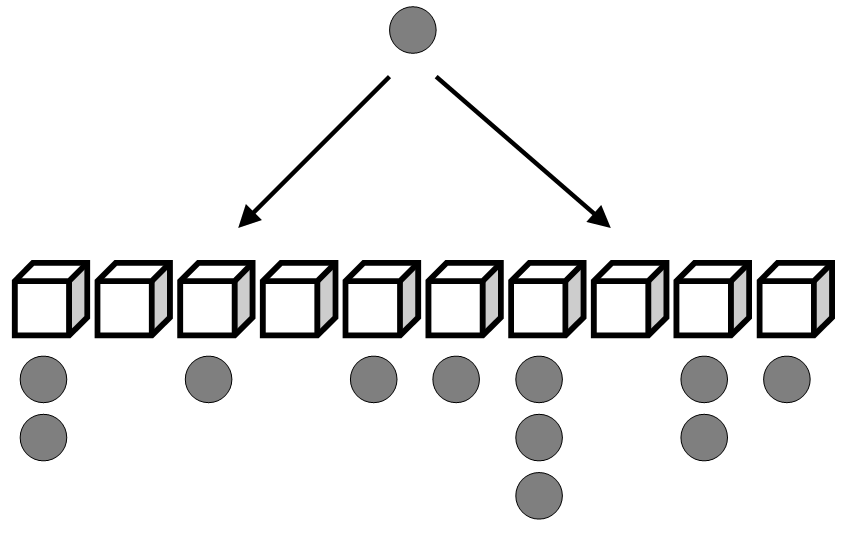
\includegraphics[width=0.7\textwidth]{two-choices.png}
		
		\caption{Two choices Insertion.}
	\end{figure}
\end{frame}

\begin{frame}
	\frametitle{Two Choices Paradigm}
	\framesubtitle{Algorithm - asymmetric tie breaking}
	
	\begin{block}{Improvement}
		\begin{itemize}
			\item Split the table into $d$ evenly sized subtables.
			\item The function $f_i(x)$ returns only bins of the $i$-th subtable.
			\item The element $x$ is placed into the leftmost least loaded bin.
			\item Leads to a better multiplicative constants in the bound.
		\end{itemize}
	\end{block}
	
	\begin{figure}
		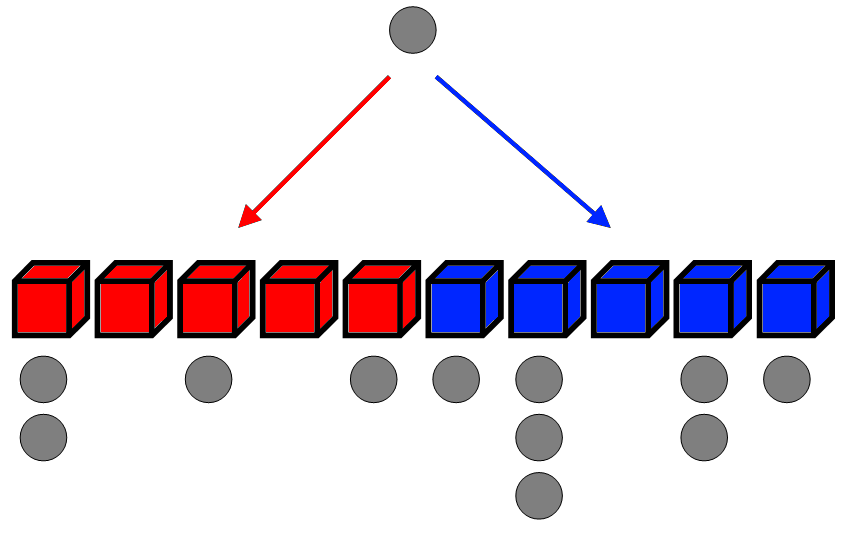
\includegraphics[width=0.3\textwidth]{two-choices-asymmetric.png}
		
		\caption{Asymmetric two choices Insertion.}
	\end{figure}
\end{frame}

\begin{frame}
	\frametitle{Two Choices Paradigm}
	\framesubtitle{Theorem}
	
	\begin{theorem}
		Assume a hash table working according to the two choices paradigm using $d$ functions. Then
		\[
			\Prob{\lpsl(S) \geq \log_d \log_2(n) + 6} = n^{-1}\left( 1 + n^{o(1)}\right) = o(1).
		\]

		If a hash table works according to the asymmetric two choices paradigm with $d$ functions, then
		\[
			\Prob{\lpsl(S) \geq \frac{\ln \log_2(n) + \ln(2)}{d \ln \phi_d} + 6} = n^{-1}\left( 1 + n^{o(1)}\right) = o(1).
		\]
	\end{theorem}
	
	Problems with dependencies with non uniform systems in case of universal hashing are solved by Woelfel's approach.
\end{frame}

\subsection{Linear hash functions}
\begin{frame}
	\frametitle{Limit function}
	\framesubtitle{Linear hash functions}
	
	Take $U$ and $V$ as fields over $\mathbb{Z}_2$. The system of all linear transformations between $U$ and $V$ provides an interesting limit function.

	\begin{theorem}
		When $n = m \log m$, then $\Expect \lpsl = \bigo(\log m \log \log m)$.
	\end{theorem}
	
	\begin{itemize}
		\item This also holds in case $n = m$ -- a consequence.
		\item Apply Markov's inequality and get that there is a constant $K$ such that $\Prob{\lpsl > K \log m \log \log m} \leq \frac{1}{2}$.
		\item Various improvements of the multiplicative constant are possible -- avoid Markov's inequality, refine the proof or assume $n = m$.
	\end{itemize}
\end{frame}

\section*{References}
\begin{frame}
	\frametitle{Literature}
	\framesubtitle{Basic methods}
	
	\begin{itemize}	
		\item Carter, J. W., Wegman, M. N.: Universal classes of hash functions, STOC '77 (1977).
		\item Fredman, M., Komlós, J., Szemerédi, E.: Storing a Sparse Table with O(1) Worst Case Access Time, Journal of the ACM (1984)
		\item Dietzfelbinger, M., Karlin, A., Mehlhorn, K., auf der Heide, F.M., Rohnert, H., Tarjan, R.E.: Dynamic perfect hashing: upper and lower bounds, Foundations of Computer Science (1988)
		\item Dietzfelbinger, M., Hühne, M., Weidlink, C.: A Dictionary Implementation Based on Dynamic Perfect Hashing, ACM Journal of Experimental Algorithmics, 2008
	\end{itemize}
\end{frame}

\begin{frame}
	\frametitle{Literature}
	\framesubtitle{Current methods}

	\begin{itemize}
		\item Arbitman, Y., Naor, M., Segev, G.: Backyard Cuckoo Hashing, FOCS (2010)
		\item Pagh, R., Rodler. F.: Cuckoo hashing, Journal of Algorithms (2004)
		\item Alon, N., Dietzfelbinger, M., Miltersen, P. B., Petrank, E. and Tardos, G.: Linear hash functions, JACM (2010)
		\item Vöcking, B.: How Asymmetry Helps Load Balancing, FOCS (1999)
		\item Woelfel, P.: Asymmetric Balanced Allocation with Simple Hash Functions, SODA (2006)
		\item Mitzenmacher, M., Richa, A. W., Sitaraman, R.: The Power of Two Random Choices: A Survey of Techniques and Results (2000)
	\end{itemize}
\end{frame}
